\section{Conceitos elementares}

\begin{frame}[fragile]{Teoria dos Conjuntos}

    \begin{block}{Termos Primitivos}
        Os termos primitivos da Teoria dos Conjuntos são:
        \begin{enumerate}
            \item elemento
            \item conjunto
        \end{enumerate}
    \end{block}

    \begin{block}{Axioma}
        Se $a$ é um elemento e $A$ é um conjunto, então ``$a$ pertence a $A$'' é uma proposição.
    \end{block}

\end{frame}

\begin{frame}[fragile]{Representação de Conjuntos}

    \textbf{Diagramas de Venn}

    \begin{figure}
        \centering

        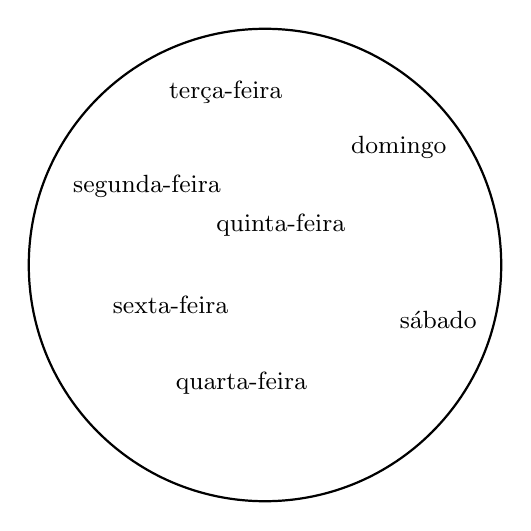
\begin{tikzpicture}
            \draw[thick] (0, 0) circle [radius=3cm];

            \node at (-1.5, 1) { \small segunda-feira };
            \node at (-0.5, 2.2) { \small terça-feira };
            \node at (-0.3, -1.5) { \small quarta-feira };
            \node at (0.2, 0.5) { \small quinta-feira };
            \node at (-1.2, -0.5) { \small sexta-feira };
            \node at (2.2, -0.7) { \small sábado };
            \node at (1.7, 1.5) { \small domingo };
        \end{tikzpicture}

        \caption{Conjunto dos dias da semana}

    \end{figure}

\end{frame}
\begin{frame}[fragile]{Representação de Conjuntos}

    \textbf{Enumeração de seus elementos}

    \vspace{0.1in}

    \begin{enumerate}
        \item Conjunto de constantes notáveis
        \[
            A = \lbrace \pi, e, 0, -1\rbrace
        \]

        \item Conjunto das notas musicais
        \[
            B = \lbrace \mbox{dó, ré, mi, fá, sol, lá, si}\rbrace
        \]

        \item Conjunto dos números primos
        \[
            C = \lbrace 2, 3, 5, 7, 11, 13, 17, \ldots \rbrace
        \]

        \item Conjuntos dos números inteiros pares
        \[
            D = \lbrace \ldots, -4, -2, 0, 2, 4, \ldots \rbrace
        \]

        \item Conjunto vazio: $\emptyset$
    \end{enumerate}
\end{frame}

\begin{frame}[fragile]{Representação de Conjuntos}

    \textbf{Propriedades de seus elementos}

    \vspace{0.1in}

    \begin{enumerate}

        \item Conjunto dos aprovados em Paradigmas de Programação:
        \[
            A = \lbrace a\in M\ |\ \mbox{média}(a) \geq 5.0 \rbrace,
        \]
        onde $M$ é o conjunto dos alunos matriculados na disciplina.

        \item Conjunto dos anos bissextos:
        \[
            B = \lbrace n\in\mathbb{N}\ |\ (4\ \mbox{divide}\ n\ \land \lnot(100\ \mbox{divide}\ 
            n)) \veebar (400\ \mbox{divide}\ n)\rbrace
        \]

        \item Conjunto dos números compostos:
        \[
            C = \lbrace n\in \mathbb{Z}\ |\ \exists\, d\in \mathbb{Z}\ \mbox{tal que}\ 1 < d < n\
                \mbox{e}\ d\ \mbox{divide}\ n\rbrace
        \]

        \item Conjunto dos divisores de $n!$:
        \[
            D(n) = \lbrace d\in \mathbb{N}\ |\ d\ \mbox{divide}\ n!\rbrace
        \]
    \end{enumerate}

\end{frame}

\begin{frame}[fragile]{Subconjuntos}

    \begin{block}{Subconjuntos}
        Seja $A$ um conjunto. Um conjunto $B$ é subconjunto de $A$ se, para qualquer $b\in B$, 
            $b\in A$. Notação: $B\subset A$.
    \end{block}

    \vspace{0.1in}

    \begin{block}{Igualdade de conjuntos}
       Dois conjuntos $A$ e $B$ são iguais se, e somente se, $A\subset B$ e $B\subset A$.
    \end{block}

\end{frame}

\begin{frame}[fragile]{Operações em conjuntos}

    \begin{block}{Operações em conjuntos}
        Sejam $A$ e $B$ dois conjuntos. São conjuntos
        \begin{enumerate}
            \item a \textbf{união}
            \[
                A \cup B = \lbrace x\ |\ x\in A\, \vee\, x\in B\rbrace
            \]

            \item a \textbf{interseção}
            \[
                A \cap B = \lbrace x\ |\ x\in A\, \land\, x\in B\rbrace
            \]

            \item a \textbf{diferença}
            \[
                A - B = \lbrace x\ |\ x\in A\, \land\, \lnot (x\in B)\rbrace
            \]
        \end{enumerate}
    \end{block}

\end{frame}
%% TODO:
% 2. Operações de conjuntos (união, interseção e diferença)
% 3. Nova aula sobre relações e funções
